%!TEX root = ./main.tex
So far, the main appeal of subjective expected utility (SEU) has been its conceptual simplicity, and the fact that it answers all decision problems in the same manner. 
In this chapter, we review some attempts at justifying SEU more formally, i.e. show that SEU logically follows from some simple, consensual principle.
When you hear someone say that ``Non-Bayesians are incoherent'', that ``a prior encapsulates the information available \emph{before} an experiment is made, so that the prior cannot depend on data", or that ``the posterior is the experimenter's updated belief after the experiment", or that ``Non-Bayesians violate the likelihood principle", they are all referring to one or the other of the formal justifications below. 
Not all these justifications are compatible, and none can really claim to be uniformly superior, so it is important to know upon what arguments you are resting your interpretation of the Bayesian procedure.

\section{Because you abide by the likelihood principle}
The ``formal" likelihood principle \citep{BeWo88} is a half-formal justification that deals primarily with the estimation problem. 
It is only half-formal because it deals with notions that are hard to rigorously define.

\subsection{The formal LP}
Consider two statistical experiments
$$
E_i=(\cY_i,\un{\theta}, \{p_i(\cdot\vert\vartheta), \vartheta\in\Theta\}), \quad i=1,2.
$$
Assume that for some realizations $\by_1$ and $\by_2$,
$$
p_1(\by_1\vert\cdot) \propto p_2(\by_2\vert \cdot).
$$
Note that we are using bold characters to insist on $\by_1$ and $\by_2$ being vectors concatenating (possibly many, of arbitrary dimension) observations, the label $i=1,2$ is only there to indicate which experiment we consider.
In particular, $\by_1$ and $\by_2$ may differ in dimension.

Now, assuming that there exists a quantity $\text{Ev}(E,x)$ that encapsulates the ``evidence on $\theta$ arising from $E$ and $x$", the formal LP principle is the requirement that
$$
\text{Ev}(E_1,\by_1) = \text{Ev}(E_2,\by_2).
$$
As a corollary, $\text{Ev}(E,\by)$ can depend on $x$ solely through $p(\by\vert\cdot)$.

\subsection{SEU satisfies the LP}
Letting $\cS = \cY^n\times\theta$, SEU satisfies the LP as long as the joint distribution over states has either $p_1$ or $p_2$ as its conditional of $\by$ given $\theta$.
Indeed, let
$$
p_i(s_i) = p_i(\by_i,\theta) = p_i(\by_i\vert\theta)\un{p(\theta)} = \un{Z} p_i(\theta\vert \by_i), \quad i=1,2.
$$
Note how we use a common prior. 
Then for $a:\cS\rightarrow\cZ$,
  $$ 
  \int L(a,s_1) \frac{p_1(\by_1\vert\theta)p(\theta)}{\un{Z}} \d\theta \propto \int L(a,s_2) \frac{p_2(\by_2\vert\theta)p(\theta)}{\un{Z}} \d\theta, 
  $$
  so that the posterior expected losses are the same in both experiments, and Bayes actions coincide.
  However, note that full expected utilities are different in general, 
  \begin{align*}
    \int L(a,s_1) p_1(\by_1\vert\theta)p(\theta) \unn{\d \by_1}\d\theta
    &\neq \int L(a,s_2) p_2(\by_2\vert\theta)p(\theta) \unn{\d \by_2}\d\theta.
  \end{align*}

\subsection{The stopping rule principle}
The same kind of computations shows that SEU with a particular choice of joint distribution is immune to data-dependent stopping rules. 
This can also be seen as a consequence of the LP \citep{BeWo88}, but we stick to SEU with some conditions on its joint distribution of states for simplicity.

Assume that we want to model the following inference problem.
We collect data one item at a time, independently from some distribution $y_i\vert\theta$, until the first $n\in\mathbb{N}$ such that $y_1,\dots,y_n \in A_n$, and then you want to estimate $\theta$. 
We model this by $\cS = \Theta \times \cup_{n\geq 1} \cY^n$, and decide to take a joint distribution $p$  such that $y_1,y_2,\dots$ are independent given $\theta$, just like we assume the data generating mechanism works. 
Then the Bayes action $a^\star = a_{g^\star}$ minimizes
\begin{align*}
   \mathbb E L(a,s) &= \mathbb E \left [ L(a,s) \sum_{n} \un{\IND{N=n}} \right ]\\
    &= \sum_{n} \mathbb E \left [ L(a,s) \un{\IND{N=N}} \right ]\\
    &= \sum_{n} \int L(a,(\theta,y_{1:n})) \un{\IND{y_{1:n}\in A_n}\prod_{k<n}\IND{y_{1:k}\notin A_k}} p(y_{1:n}\vert\theta) p(\theta) \d y_{1:n}\d \theta.\\
    &= \sum_n \int\d y_{1:n} \un{\IND{y_{1:n}\in A_n}\prod_{k<n}\IND{y_{1:k} \notin A_k}} \int  L(a,(\theta,y_{1:n}))  p(y_{1:n}\vert\theta) p(\theta),
\end{align*}
where we used the monotone convergence theorem and Fubini's theorem (assuming, e.g., that the loss is bounded).
So, to find the minimizer $g^\star$ defined on $\cup_n \cY^n$ of the overall expected loss, it is enough, for each $n$, to define $g^\star(y_{1:n})$ as the usual Bayes rule for fixed $n$, i.e. as the minimizer of the inner integral.
In other words, as long as the prior $p(\theta)$ does not depend on data, the Bayes decision is immune to data-dependent stopping rules: just act as if there were no stopping rule.

\subsection{Pros and cons of the LP}
\begin{itemize}
  \item The LP is compelling to many \citep{BeWo88}, but it has its downsides.
  \item Being Bayesian is not the only way to abide by the LP.
  \item I am personally uncomfortable with the stopping rule principle, probably because my frequentist intuition is still too strong.
  \item It is hard to make fully formal: is $\text{Ev}(E,x)$ even meaningful? See answer by LeCam to \citep{BeWo88}.
  \item It assumes we want to specify a likelihood, this prevents model-free Bayesianism.
  \item It separates the roles of the likelihood and the prior. For LP-abiding Bayesians, \un{the prior is not allowed to depend on data}.
\end{itemize}

% % ###############################################
\section{Because you place coherence above all things: subjective Bayes}
% % ###############################################

% % ###############################################
\section{Because you like coherence and consensus: objective Bayes}
% % ###############################################

% % ###############################################
\section{Because you are a Waldian frequentist in disguise}
% % ###############################################

\subsection{On the consistency of Bayesian estimators}

\subsection{Complete class theorems}

\subsection{PAC-Bayes statistical learning}


% \begin{frame}
%   \frametitle{The subjectivistic viewpoint}
%   \begin{itemize}
%     \item Top requirement is \un{internal coherence} of decisions.
%     \item Various attempts at proving that, internally, coherent decision makers minimize some expected utility; see \citep{PaIn09}.
%     \begin{figure}
%       \centering
%       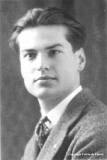
\includegraphics[width=\threefig]{\figdir/deFinetti.jpg}
%       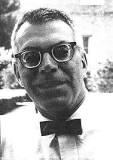
\includegraphics[width=\threefig]{\figdir/savage.jpg}
%       \caption{Bruno de Finetti (1906--1985) and L. ``Jimmie" Savage (1917--1971)}
%     \end{figure}
%   \end{itemize}
% \end{frame}

% \begin{frame}{Savage's axioms}
% \begin{itemize}
% \item Start with the triple $(\cS,\cZ,\cA\subset \cF(\cS, \cZ))$ as in \cite{Wal50}.
% \item Savage's idea is to list what we expect from a binary relation $\prec$ on $\cA\times \cA$ describing a decision maker's preferences.
% \end{itemize}
% \blank
% \blank
% \end{frame}

% \begin{frame}{Savage's axioms}
% \end{frame}

% \begin{frame}{Savage's axioms}
% \end{frame}

% \begin{frame}{A De Finetti theorem by Hewitt \& Savage}
%   \begin{block}{Theorem; see \citep[Theorem 1.49]{Sch12}}
%     Let $X_1,X_2,\dots$ be a sequence of exchangeable random variables on $\cX$, i.e.
%     $$
%     X_1,\dots,X_n \sim X_{\pi(1)},\dots, X_{\pi(n)}, \forall n, \forall \pi\in\frak S_n.
%     $$
%     Then there exists a probability distribution $\mu$ \un{on the set of probability measures $\mathcal P(\cX)$ on $\cX$} such that
%     $$
%     \mathbb P (X_1\in A_1, \dots, X_n\in A_n) = \int Q(A_1)\dots Q(A_n)\d\mu(Q).
%     $$
%     % Furthermore, for each $A$,
%     % $$
%     % Q(A) = \lim_{n\rightarrow\infty} \frac 1n\sum_{i=1}^n 1_A(X_i)\quad a.s.
%     % $$
%   \end{block}
%   \vfill
%   To a subjectivist, Savage's theorem says you should use SEU, and representation theorems like de Finetti's constrain your choice of $p$.
% \end{frame}

% % \begin{frame}{De Finetti's theorem and LDA}
% % \end{frame}

% % \begin{frame}{De Finetti's theorem and Bayesian nonparametrics}
% % \end{frame}

% \begin{frame}{Bonus: The Dirichlet process through de Finetti's theorem}

% \begin{block}{The Blackwell-McQueen urn scheme (aka the CRP)}
%   Start with an urn containing a single black ball with weight $\alpha$. Repeat: draw a ball from the urn with probability $\propto$ its weight. Then,
%   \begin{itemize}
%     \item If the ball is black, return it to the urn along with another ball of weight 1, with a \un{new color} sampled from some base measure $H$.
%     \item If the ball is colored, return it to the urn along with another ball of weight 1 of the \un{same color}.
%   \end{itemize}
%   Denote by $X_1, X_2, \dots$ the color of the ball added.
% \end{block}
% \begin{flushright}
%   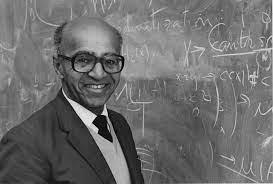
\includegraphics[width=\twofigminus]{Figures/blackwell.jpg}
% \end{flushright}
% \vfill
% % \begin{itemize}
% %   \item Exercise: show that $X_1,X_2,...$ are exchangeable.
% %   \item The corresponding prior $\mu$ on $\mathcal{P}(\cX)$ is the Dirichlet process with concentration $\alpha$ and base measure $H$.
% % \end{itemize}
% \end{frame}

% \begin{frame}{Pros and cons of the subjectivist viewpoint}
% \begin{itemize}
%   \item Axiomatic derivations are powerful, and shed light on what coherence requires. \un{In particular, coherence leads to SEU}.
%   \vfill
%   \item[\frownie] ... Yet all axiomatic systems have a bit that is difficult to swallow.
%   \vfill
%   \item Priors should be elicited by \un{expert knowledge}, and should be \emph{bona fide} probability distributions.
%   \vfill
%   \item Representation theorems can help design the joint distribution over states \citep{OrRo14}.
%   \vfill
%   \item Bayesian nonparametrics has revived the subjectivist viewpoint.
% \end{itemize}

% \end{frame}
